\likechapter{Приложение А}

\renewcommand{\thetable}{\textmd{A.}\arabic{table}}
\setcounter{table}{0}
\begin{table}[ht!]
	\small
    \caption{Классификация неровностей поверхности и рельефа \cite{mlyavaya}.}
    \label{table_z0}
	\setlength{\extrarowheight}{0.5mm}
	\centering
    \begin{tabular}{|M{0.03\textwidth}|M{0.5\textwidth}|M{0.18\textwidth}|M{0.18\textwidth}|}
    \hline № & Вид поверхности & Класс неровности рельефа K & Размер шероховатости $Z_0$ \\
    
    \hline 1. & Водная поверхность (море, озеро); снежная поверхность & 0 & \makecell{0,02 см \\ 0,05-0,1 см} \\
    
    \hline 2. & Полностью открытый рельеф с гладкой поверхностью (взлетные полосы, ровные поля, скошенная трава) & 
    	0,5 & 0,24-0,5 см \\
    
    \hline 3. & Открытые области с небольшими лесозащитными полосами (равнины или небольшие холмы, пашня, травяные 
    	поля); небольшие фермерские постройки, отдельно стоящие деревья или кустарники & 1 & 1-3 см \\
    
    \hline 4. & Ровная, слегка холмистая местность, сельскохозяйственные угодья (поле с высокой растительностью, 
    	пшеничное поле) с несколькими зданиями и навесами высотой до 8 м, расположенными друг от друга на расстоянии 
    	около 1250 м & 0 & 5 см\\
    
    \hline 5. & Ровная или слегка холмистая территория, хозяйственные земли с разбросанными областями построек и 
    	небольшими лесозащитными полосами, среднее расстояние между которыми составляет 1000 м & 2 & 10 см \\
    
    \hline 6. & Сельскохозяйственные угодья с большим количеством зданий или навесами высотой до 8 м, с деревьями, 
    	кустарниками, расположенными друг от друга на расстоянии около 250 м & 2,5 & 20-25 см \\
    
    \hline 7. & Территории с очень неровным рельефом, городские застройки, леса или сельскохозяйственные земли с 
    	многочисленными близкорасположенными лесозащитными полосами, среднее расстояние между которыми составляет 
    	несколько сотен метров; болота с растительностью 
    	& 3 & \makecell{40 см \\ 60 см} \\

    \hline 8. & Города с высокими зданиями & 3,5 & 80-150 см \\
    
    \hline 9. & Большие города, мегаполисы с высокими зданиями и небоскребами & 4 & 160-200 см \\

    \hline
    \end{tabular}
\end{table}

\clearpage

\likechapter{Приложение Б}

\renewcommand{\thetable}{\textmd{Б.}\arabic{table}}
\setcounter{table}{0}
\begin{table}[ht]
    \small
    \caption{Основные характеристики радионуклидов, образующися в топливе.}
    \label{table_tvel_radio}
    \setlength{\extrarowheight}{0.5mm}
    \centering
    \begin{tabular}{|M{0.225\textwidth}|M{0.225\textwidth}|M{0.225\textwidth}|M{0.225\textwidth}|}
    \hline Нуклид & $A_{i}^{0}$, Бк/кг & $Z_i$ & $\gamma_{i}$ \\

    \hline I-131 & $3,000 \times 10^6$ & $6,0$ & $2,88 \times 10^{-2}$ \\
    \hline I-132 & $2,072 \times 10^6$ & $1,0$ & $1,15 \times 10^{-2}$ \\ 
    \hline I-133 & $6,290 \times 10^5$ & $1,0$ & $6,70 \times 10^{-2}$ \\
    \hline I-134 & $3,700 \times 10^6$ & $1,0$ & $3,93 \times 10^{-2}$ \\
    \hline I-135 & $1,590 \times 10^6$ & $1,0$ & $6,28 \times 10^{-2}$ \\

    \hline Cs-134 & $7,770 \times 10^2$ & $1,0$ & $7,71 \times 10^{-8}$ \\
    \hline Cs-137 & $1,600 \times 10^4$ & $1,0$ & $6,23 \times 10^{-2}$ \\
    \hline Cs-138 & $4,100 \times 10^5$ & $0,2$ & Продукт распада Xe-138 \\

    \hline Rb-88 & $4,100 \times 10^5$ & $4,0$ & Продукт распада Kr-88 \\

    \hline Xe-133 & $2,500 \times 10^5$ & $19,0$ & $6,70 \times 10^{-2}$ \\
    \hline Xe-135 & $2,738 \times 10^6$ & $1,0$ & $2,68 \times 10^{-3}$ \\
    \hline Xe-137 & $1,406 \times 10^6$ & $1,0$ & $7,74 \times 10^{-2}$ \\
    \hline Xe-138 & $1,600 \times 10^5$ & $3,0$ & $1,20 \times 10^{-2}$ \\
    
    \hline Kr-85 & $2,500 \times 10^5$ & $1,0$ & $1,30 \times 10^{-2}$ \\
    \hline Kr-87 & $7,030 \times 10^5$ & $1,0$ & $3,64 \times 10^{-2}$ \\
    \hline Kr-88 & $1,600 \times 10^5$ & $4,0$ & $3,64 \times 10^{-2}$ \\

    \hline H-3 & $3,700 \times 10^7$ & $1,0$ & $1,70 \times 10^{-9}$ \\
    \hline
    \end{tabular}
\end{table}

\clearpage

\likechapter{Приложение В}

\renewcommand{\thefigure}{\textmd{В.}\arabic{figure}}
\setcounter{figure}{0}

\begin{figure}[ht]
\centering
    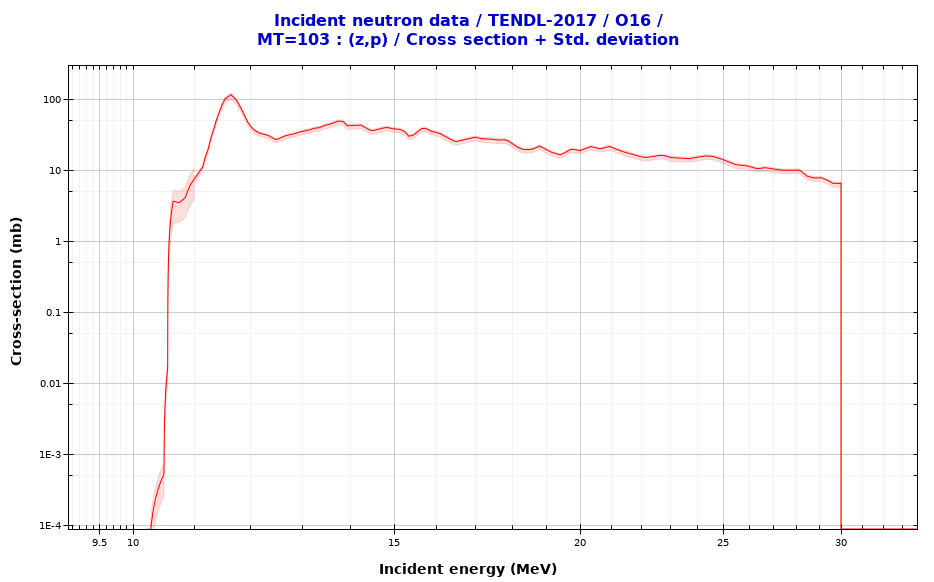
\includegraphics[height=7.9cm]{O16_np_cross}
    \captionsetup{justification=centering}
    \caption{Энергетическая зависимость микроскопического сечения реакции (n, p) на ядре $^{16}\text{O}$ \cite{janis}.}
    \label{fig_O16_cross}
\end{figure}

\begin{figure}[ht]
\centering
    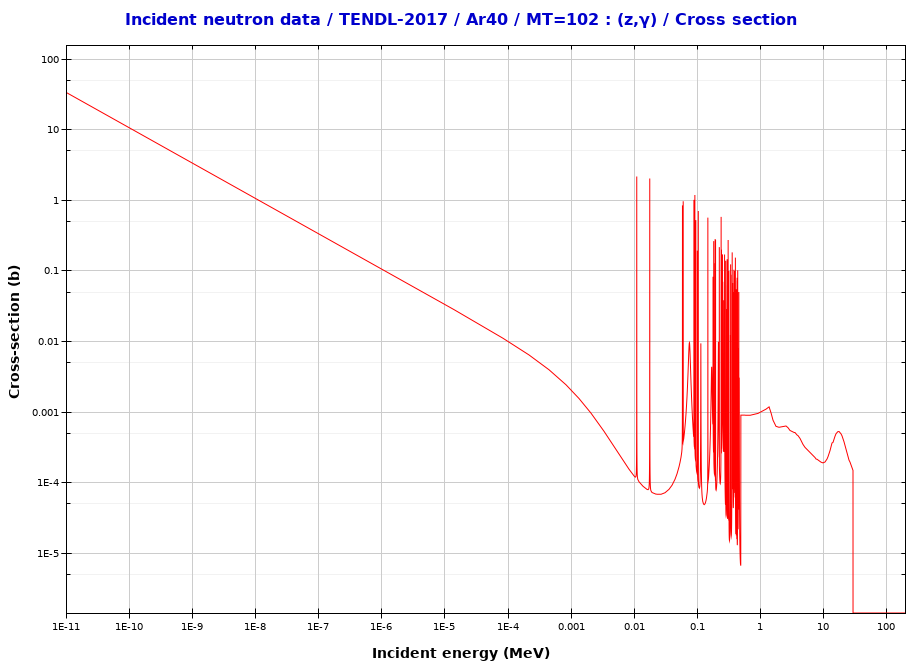
\includegraphics[height=7.9cm]{Ar40_ngamma_cross}
    \captionsetup{justification=centering}
    \caption{Энергетическая зависимость микроскопического сечения реакции (n, $\gamma$) на ядре $^{40}\text{Ar}$ \cite{janis}.}
    \label{fig_Ar40_cross}
\end{figure}

\begin{figure}[ht]
\centering
    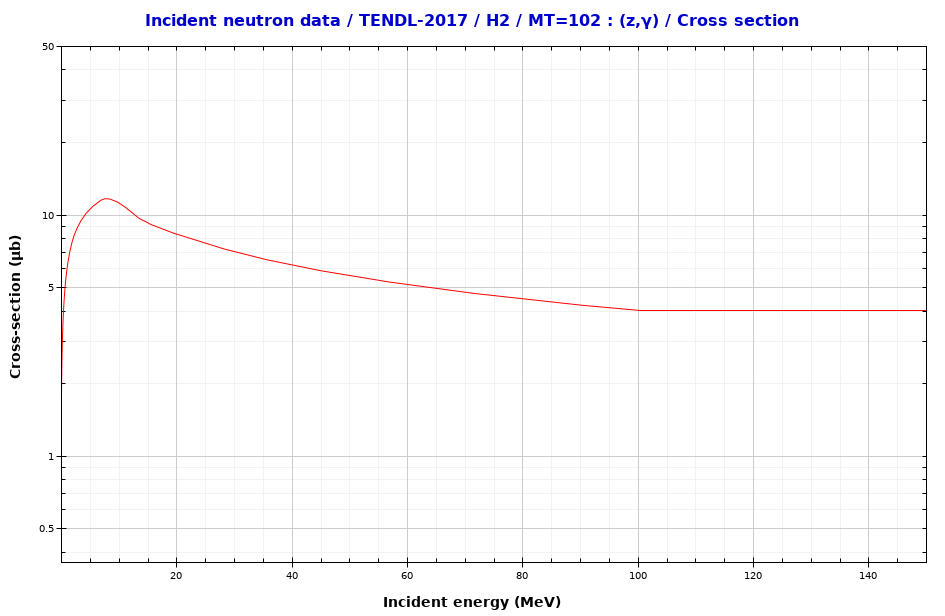
\includegraphics[height=7.9cm]{H2_ngamma_cross}
    \captionsetup{justification=centering}
    \caption{Энергетическая зависимость микроскопического сечения реакции (n, $\gamma$) на ядре $^{2}\text{H}$ \cite{janis}.}
    \label{fig_H2_cross}
\end{figure}